\documentclass{standalone}
\usepackage{tikz}
\usetikzlibrary{positioning}

\begin{document}

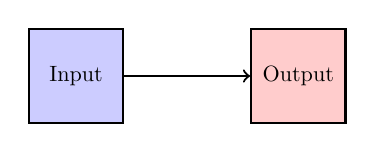
\begin{tikzpicture}[thick,scale=0.8, every node/.style={transform shape}]

% Definir nodos de la red neuronal
\node[draw=black,fill=blue!20,minimum size=1.5cm] (input) at (0,0) {Input};
\node[draw=black,fill=red!20,minimum size=1.5cm,right=2cm of input] (output) {Output};

% Conexiones entre nodos
\draw[->] (input) -- (output);

\end{tikzpicture}

\end{document}
